\begin{figure}
    \centering

    \begin{subfigure}{0.8\columnwidth}
        \centering
        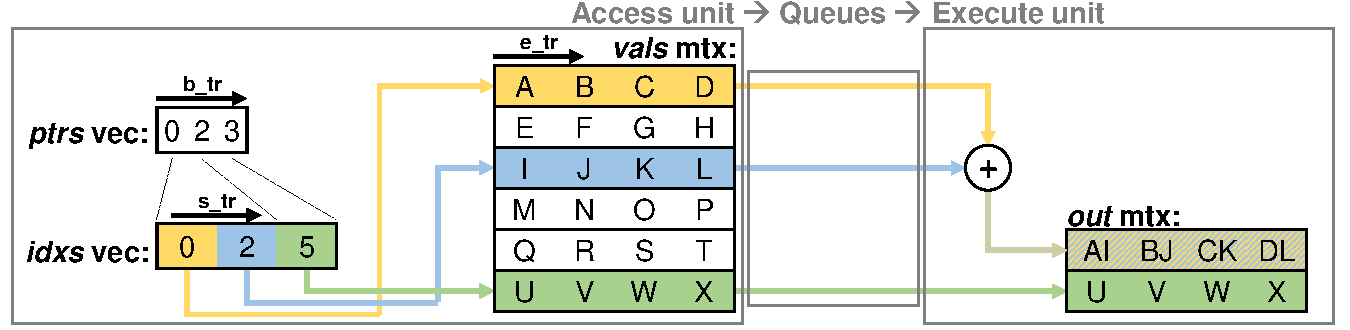
\includegraphics[width=\linewidth]{img_sls_example.pdf}
        \caption{Functional example of the EB function.}
        \label{fig:eb-functional-example}
    \end{subfigure}
    
    \begin{minipage}{\columnwidth}
    \begin{lstlisting}[xleftmargin=8pt]
void eb(idxs, ptrs, vals, out){
  for(int b = 0; b < num_batches; b++){ // Batch traversal (b_tr)
    for(int p = ptrs[b]; p < ptrs[b+1]; p++){ // Segment traversal (s_tr)
      idx = idxs[p]; // Load embedding index
      for(int e = 0; e < emb_len; e++){ // Embedding vec traversal (e_tr)
        val = vals[p,e]; // Load embedding element
        out[b,e] += val; }}}} // Reduce embedding elements
    \end{lstlisting}
    \vspace{-0.5em}
    \subcaption{Traditional imperative code, which also acts as input to Ember.}
    \label{fig:eb-imperative-code}
    \end{minipage}

    \begin{minipage}{\columnwidth}
    \begin{lstlisting}[xleftmargin=8pt]
 tr b_tr=loop_tr(0, num_batches, 1) // iterate thru batch
 str beg_ptr=b_tr.mem_str(ptrs, b_tr.ite) // load segment beg ptr
 str end_pos=b_tr.alu_str('+', b_tr.ite, 1) // compute next ptr pos
 str end_ptr=b_tr.mem_str(ptrs, end_pos) // load segment end ptr

 tr s_tr=loop_tr(beg_ptr, end_ptr, 1) // iterate thru segment
 str emb_idx=s_tr.mem_str(s_tr, idxs, s_tr.ite) // load emb idx
 str emb_beg=s_tr.alu_str(s_tr, '*', emb_idx, emb_len) // emb addr

 tr e_tr=loop_tr(0, emb_len, 1) // iterate thru emb vec
 str emb_pos=alu_str('+', emb_beg, e_tr.ite) // element addr
 str emb_val=mem_str(vals, emb_pos) // load emb element

 enq_op(b_tr.ite, e_tr, ite) // push batch position
 enq_op(e_tr.ite, e_tr, ite) // push emb el position
 enq_op(emb_val, e_tr, ite) // push emb el value
 callback(e_tr, ite) //trigger call on every emb iter
    \end{lstlisting}
    \vspace{-0.5em}
    \subcaption{DLC dataflow lookup code.}
    \label{fig:dlc-lookup-code}
    \end{minipage}
    
    \begin{subfigure}{\columnwidth}
        \centering
        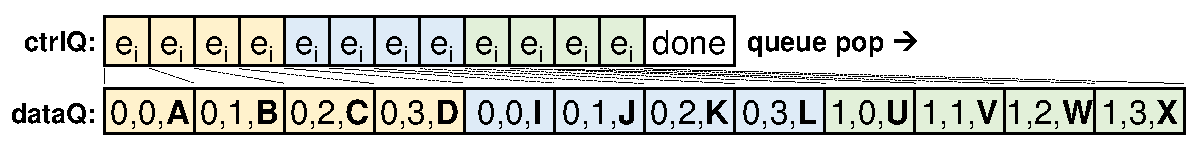
\includegraphics[width=0.81\columnwidth]{img_sls_queue.pdf}
        \caption{DLC queue content for the EB example.}
        \label{fig:dlc-queue-content}
    \end{subfigure}
    
    \begin{minipage}{\columnwidth}
    \begin{lstlisting}[xleftmargin=8pt]
while(ctrlQ.pop() == (*$e_i$*)){ // while some element
  b = dataQ.pop<1 x i32>(); // read embedding position
  e = dataQ.pop<1 x i32>(); // read element position
  v = dataQ.pop<1 x f32>(); // read element value
  fma(&out[b,e],v); // compute and store
    \end{lstlisting}
    \vspace{-0.5em}
    \subcaption{DLC imperative compute code.}
    \label{fig:dlc-compute-code}
    \end{minipage}
    %\vspace{-0.5em} % Adds vertical spacing between subfigures
    \caption[DLC representation of an EB operation.]{DLC representation of an EB operation. The functional example and imperative code define the source computation, the lookup code traverses batches, segments, and embedding elements with streams, the queues serialize callback tokens and operands, and the compute code dequeues those values to update the output. Overall, DLC separates embedding lookup from accumulation while preserving the callback order of the original loop nest.}
    \label{fig:dlc-eb-abstraction}
\end{figure}
